\documentclass[tikz,border=10pt]{standalone}
\usepackage[T1]{fontenc}
\usepackage{inter}
\renewcommand{\familydefault}{\sfdefault}
\usepackage{tikz}
\usetikzlibrary{arrows.meta, shapes.geometric, positioning, fit, backgrounds, calc, shadows}

% --- Colour palette ---
\definecolor{accent-warm}{HTML}{E57222}
\definecolor{ink}{HTML}{434343}
\definecolor{muted}{HTML}{999999}
\definecolor{platform-bg}{HTML}{FDF6F0}
\definecolor{accent-cool}{HTML}{3B7DD8}
\definecolor{eco-tone}{HTML}{0C6652}
\definecolor{cust-tone}{HTML}{014B38}

\begin{document}
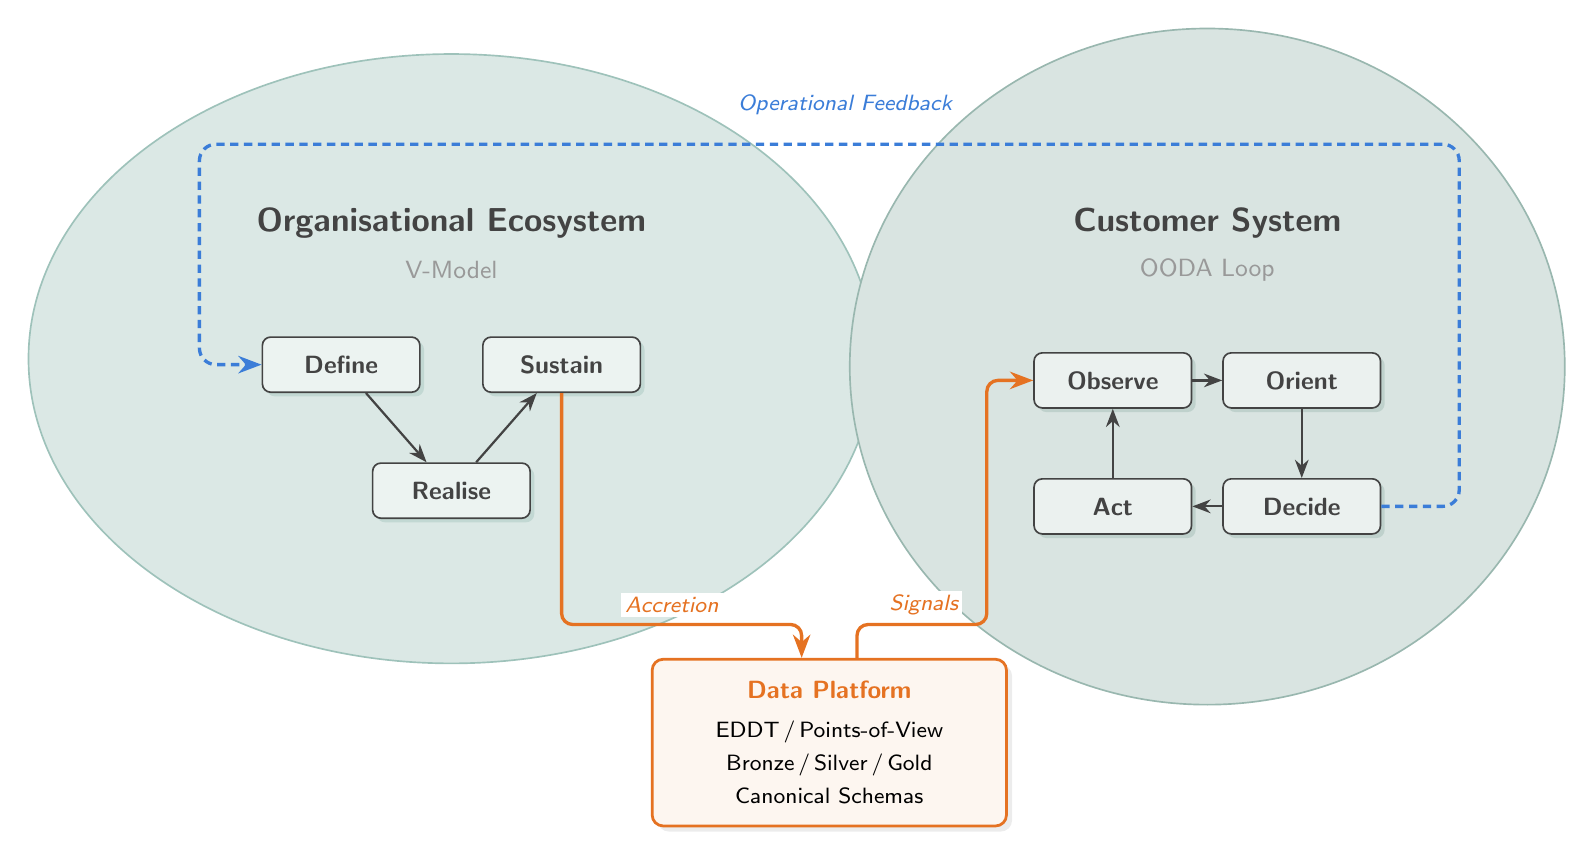
\begin{tikzpicture}[
    font=\small,
    >=Stealth,
    % Shadow colour uses xcolor mixing (e.g. eco-tone!25 = 25% teal + 75% white)
    % rather than fill opacity, because dvisvgm pre-composites transparency
    % during PDF→SVG conversion — baking the shadow as a solid fill. Mixing
    % the lobe colour with white simulates opacity while keeping consistent
    % shadow appearance in both PDF and SVG. Each lobe's shadows are tinted
    % to match their parent colour; the platform uses neutral grey.
    phase/.style={
        rectangle, rounded corners=3pt,
        minimum width=2.0cm, minimum height=0.7cm,
        draw=ink, line width=0.6pt,
        fill=white,
        font=\small\bfseries,
        text=ink,
    },
    eco-phase/.style={
        phase, fill=eco-tone!8,
        drop shadow={shadow xshift=1.5pt, shadow yshift=-1.5pt, color=eco-tone!35},
    },
    cust-phase/.style={
        phase, fill=cust-tone!8,
        drop shadow={shadow xshift=1.5pt, shadow yshift=-1.5pt, color=cust-tone!35},
    },
    lobetitle/.style={font=\large\bfseries, text=ink},
    patsub/.style={font=\small, text=muted},
    platform/.style={
        rectangle, rounded corners=4pt,
        draw=accent-warm, line width=1pt,
        fill=platform-bg,
        inner sep=8pt, align=center,
        drop shadow={shadow xshift=2pt, shadow yshift=-2pt, color=black!15},
    },
    elabel/.style={font=\footnotesize\itshape, text=accent-warm, fill=white, inner sep=1.5pt},
    flabel/.style={font=\footnotesize\itshape, text=accent-cool, inner sep=1.5pt},
    flow/.style={->, thick, ink},
    bridge/.style={->, very thick, accent-warm},
    feedback/.style={->, very thick, accent-cool, densely dashed},
]

% =====================================================================
% LEFT LOBE — Organisational Ecosystem (V-Model)
% =====================================================================

\node[lobetitle] (LT) at (-4.8, 5.4) {Organisational Ecosystem};
\node[patsub]    (LP) at (-4.8, 4.8) {V-Model};

% V shape: Define (top-left) → Realise (bottom) → Sustain (top-right)
\node[eco-phase] (define)  at (-6.2, 3.6) {Define};
\node[eco-phase] (realise) at (-4.8, 2.0) {Realise};
\node[eco-phase] (sustain) at (-3.4, 3.6) {Sustain};

\draw[flow] (define)  -- (realise);
\draw[flow] (realise) -- (sustain);

\begin{scope}[on background layer]
    \node[
        fit=(define)(realise)(sustain)(LT),
        ellipse,
        draw=eco-tone!40, line width=0.6pt,
        fill=eco-tone!15,
        inner xsep=1.2cm, inner ysep=0.7cm,
    ] (lobeL) {};
\end{scope}

% =====================================================================
% RIGHT LOBE — Customer System (OODA Loop)
% =====================================================================

\node[lobetitle] (RT) at (4.8, 5.4) {Customer System};
\node[patsub]    (RP) at (4.8, 4.8) {OODA Loop};

\node[cust-phase] (observe) at (3.6, 3.4) {Observe};
\node[cust-phase] (orient)  at (6.0, 3.4) {Orient};
\node[cust-phase] (decide)  at (6.0, 1.8) {Decide};
\node[cust-phase] (act)     at (3.6, 1.8) {Act};

\draw[flow] (observe) -- (orient);
\draw[flow] (orient)  -- (decide);
\draw[flow] (decide)  -- (act);
\draw[flow] (act)     -- (observe);

\begin{scope}[on background layer]
    \node[
        fit=(observe)(orient)(decide)(act)(RT),
        ellipse,
        draw=cust-tone!40, line width=0.6pt,
        fill=cust-tone!15,
        inner xsep=1.0cm, inner ysep=0.9cm,
    ] (lobeR) {};
\end{scope}

% =====================================================================
% DATA PLATFORM — centred at x=0
% =====================================================================

\node[platform, minimum width=4.5cm] (plat) at (0, -1.2) {
    \textbf{\textcolor{accent-warm}{Data Platform}}\\[3pt]
    {\footnotesize \mbox{EDDT\,/\,Points-of-View}}\\[1pt]
    {\footnotesize \mbox{Bronze\,/\,Silver\,/\,Gold}}\\[1pt]
    {\footnotesize Canonical Schemas}
};

% =====================================================================
% ACCRETION: Sustain → down → horizontal at y=0.3 → down into Platform
% =====================================================================

% Explicit rectilinear: vertical, horizontal, vertical
\draw[bridge, rounded corners=4pt]
    (sustain.south)
    -- (sustain.south |- 0, 0.3)          % down to shared horizontal level
    -- ([xshift=-10pt] plat.north |- 0, 0.3) % horizontal to platform entry x
    -- ([xshift=-10pt] plat.north);       % down into platform
\node[elabel] at (-2.0, 0.55) {Accretion};

% =====================================================================
% SIGNALS: Platform → up → left (clear Act) → up → right into Observe
% =====================================================================

\draw[bridge, rounded corners=4pt]
    ([xshift=10pt] plat.north)
    -- ([xshift=10pt] plat.north |- 0, 0.3)  % up to shared horizontal level
    -- (2.0, 0.3)                              % horizontal left, clearing Act
    -- (2.0, 3.4)                              % up to Observe's y level
    -- (observe.west);                         % right into Observe
\node[elabel] at (1.2, 0.55) {Signals};

% =====================================================================
% OPERATIONAL FEEDBACK: Decide → right → up → across top → down → Define
% Feedback originates from the customer system and arcs over both lobes,
% visually bridging the two as a continuous cycle.
% =====================================================================

\draw[feedback, rounded corners=6pt]
    (decide.east)
    -- (8.0, 1.8)
    -- (8.0, 6.4)
    -- (-8.0, 6.4)
    -- (-8.0, 3.6)
    -- (define.west);
\node[flabel] at (0.2, 6.9) {Operational Feedback};

\end{tikzpicture}
\end{document}
